\section{Background: Domain-specific languages in a nutshell}
\label{sec:background}

\subsubsection{Specification.} Like general purpose languages (GPLs), DSLs are defined in terms of syntax and semantics \cite{Harel:2004b}. Hence, the specification of a DSL is a tuple $<syn,sem,M_{syn\leftarrow sem}>$ \cite{Combemale:2013}. The parameter $syn$ (the \textit{\textbf{syn}tax}) refers to the structure of the DSL and specifies each language construct in terms of its name and the relationships it has with other language constructs. In turn, the parameter $sem$ (the \textit{\textbf{sem}antics}) refers to the meaning of the language constructs. This meaning corresponds to the dynamic behavior that establishes the manner in which language constructs are manipulated at runtime. Finally, the parameter $M_{syn\leftarrow sem}$ refers to the mapping between the language constructs and the semantics. 
 

\vspace{-3mm}
\subsubsection{Technological space.} Currently, there are diverse technological spaces available for the implementation of syntax and semantics of DSLs \cite{Mernik:2005b}. Language designers can, for example, choose between using context-free grammars or metamodels as specification formalism for syntax. Similarly, there are at least three technological spaces for expressing semantics: operationally, denotationally, and axiomatically \cite{Mosses:2001}.

In this paper we are interested on executable DSLs (xDSLs) which syntax is specified by means of metamodels and semantics is specified operationally as a set methods (a.k.a, \textit{domain-specific actions} \cite{Combemale:2013}). Each language construct is specified in a metaclass. The relationships between language constructs are specified as references between metaclasses. In turn, domain-specific actions are specified as java-like methods that are allocated in the metaclasses.
 
\vspace{-3mm}
\subsubsection{Implementation.} In order to implement a DSL, language designers need tool sets that offer capabilities to specify a DSL according to the selected technological space. This kind of tool sets are commonly implemented as language workbenches (such as Eclipse Modeling Framework \cite{Steinberg:2009} or MetaEdit+ \cite{Kelly:2013}) that provide meta-languages for where syntax and semantics can be expressed.

The ideas presented in this paper are implemented in an Eclipse-based language workbench. Metamodels are specified in the Ecore language whereas domain-specific actions are specified as methods in Xtend programming language\footnote{\url{http://www.eclipse.org/xtend/}}. The mapping between metaclasses and domain-specific actions is specified by using the notion of aspect introduced by the Kermeta 3\footnote{\url{https://github.com/diverse-project/k3/wiki/Defining-aspects-in-Kermeta-3}} and Melange\footnote{\url{http://melange-lang.org/}} as explained in \cite{degueule:2015}. 

\vspace{-3mm}
\subsubsection{Example: A DSL for finite state machines.} Let us illustrate executable DSLs by means of a simple example. Consider the metamodel for a simple language for finite state machines introduced at the top of Figure \ref{fig:k3-example}. It contains thee classes \texttt{StateMachine}, \texttt{State}, and \texttt{Transition}; The class \texttt{StateMachine} contains both states and transitions which is represented with containment references.

The code snippets at the bottom of Figure \ref{fig:k3-example} introduce some operational semantics to this metamodel by using K3. Note that the main feature of K3 is the notion of aspect that permits to weave the operational semantics defined in a Xtend class to a metamodel defined in Ecore. In our example, the metaclass \texttt{StateMachine} is enriched with the operation \texttt{eval()} that contains a loop that sequentially invokes the operation defined for the class \texttt{State}. This operation is also defined by using one aspect. The metaclass \texttt{Transition} is enriched with the operation \texttt{fire()}.

\begin{figure}
\centering
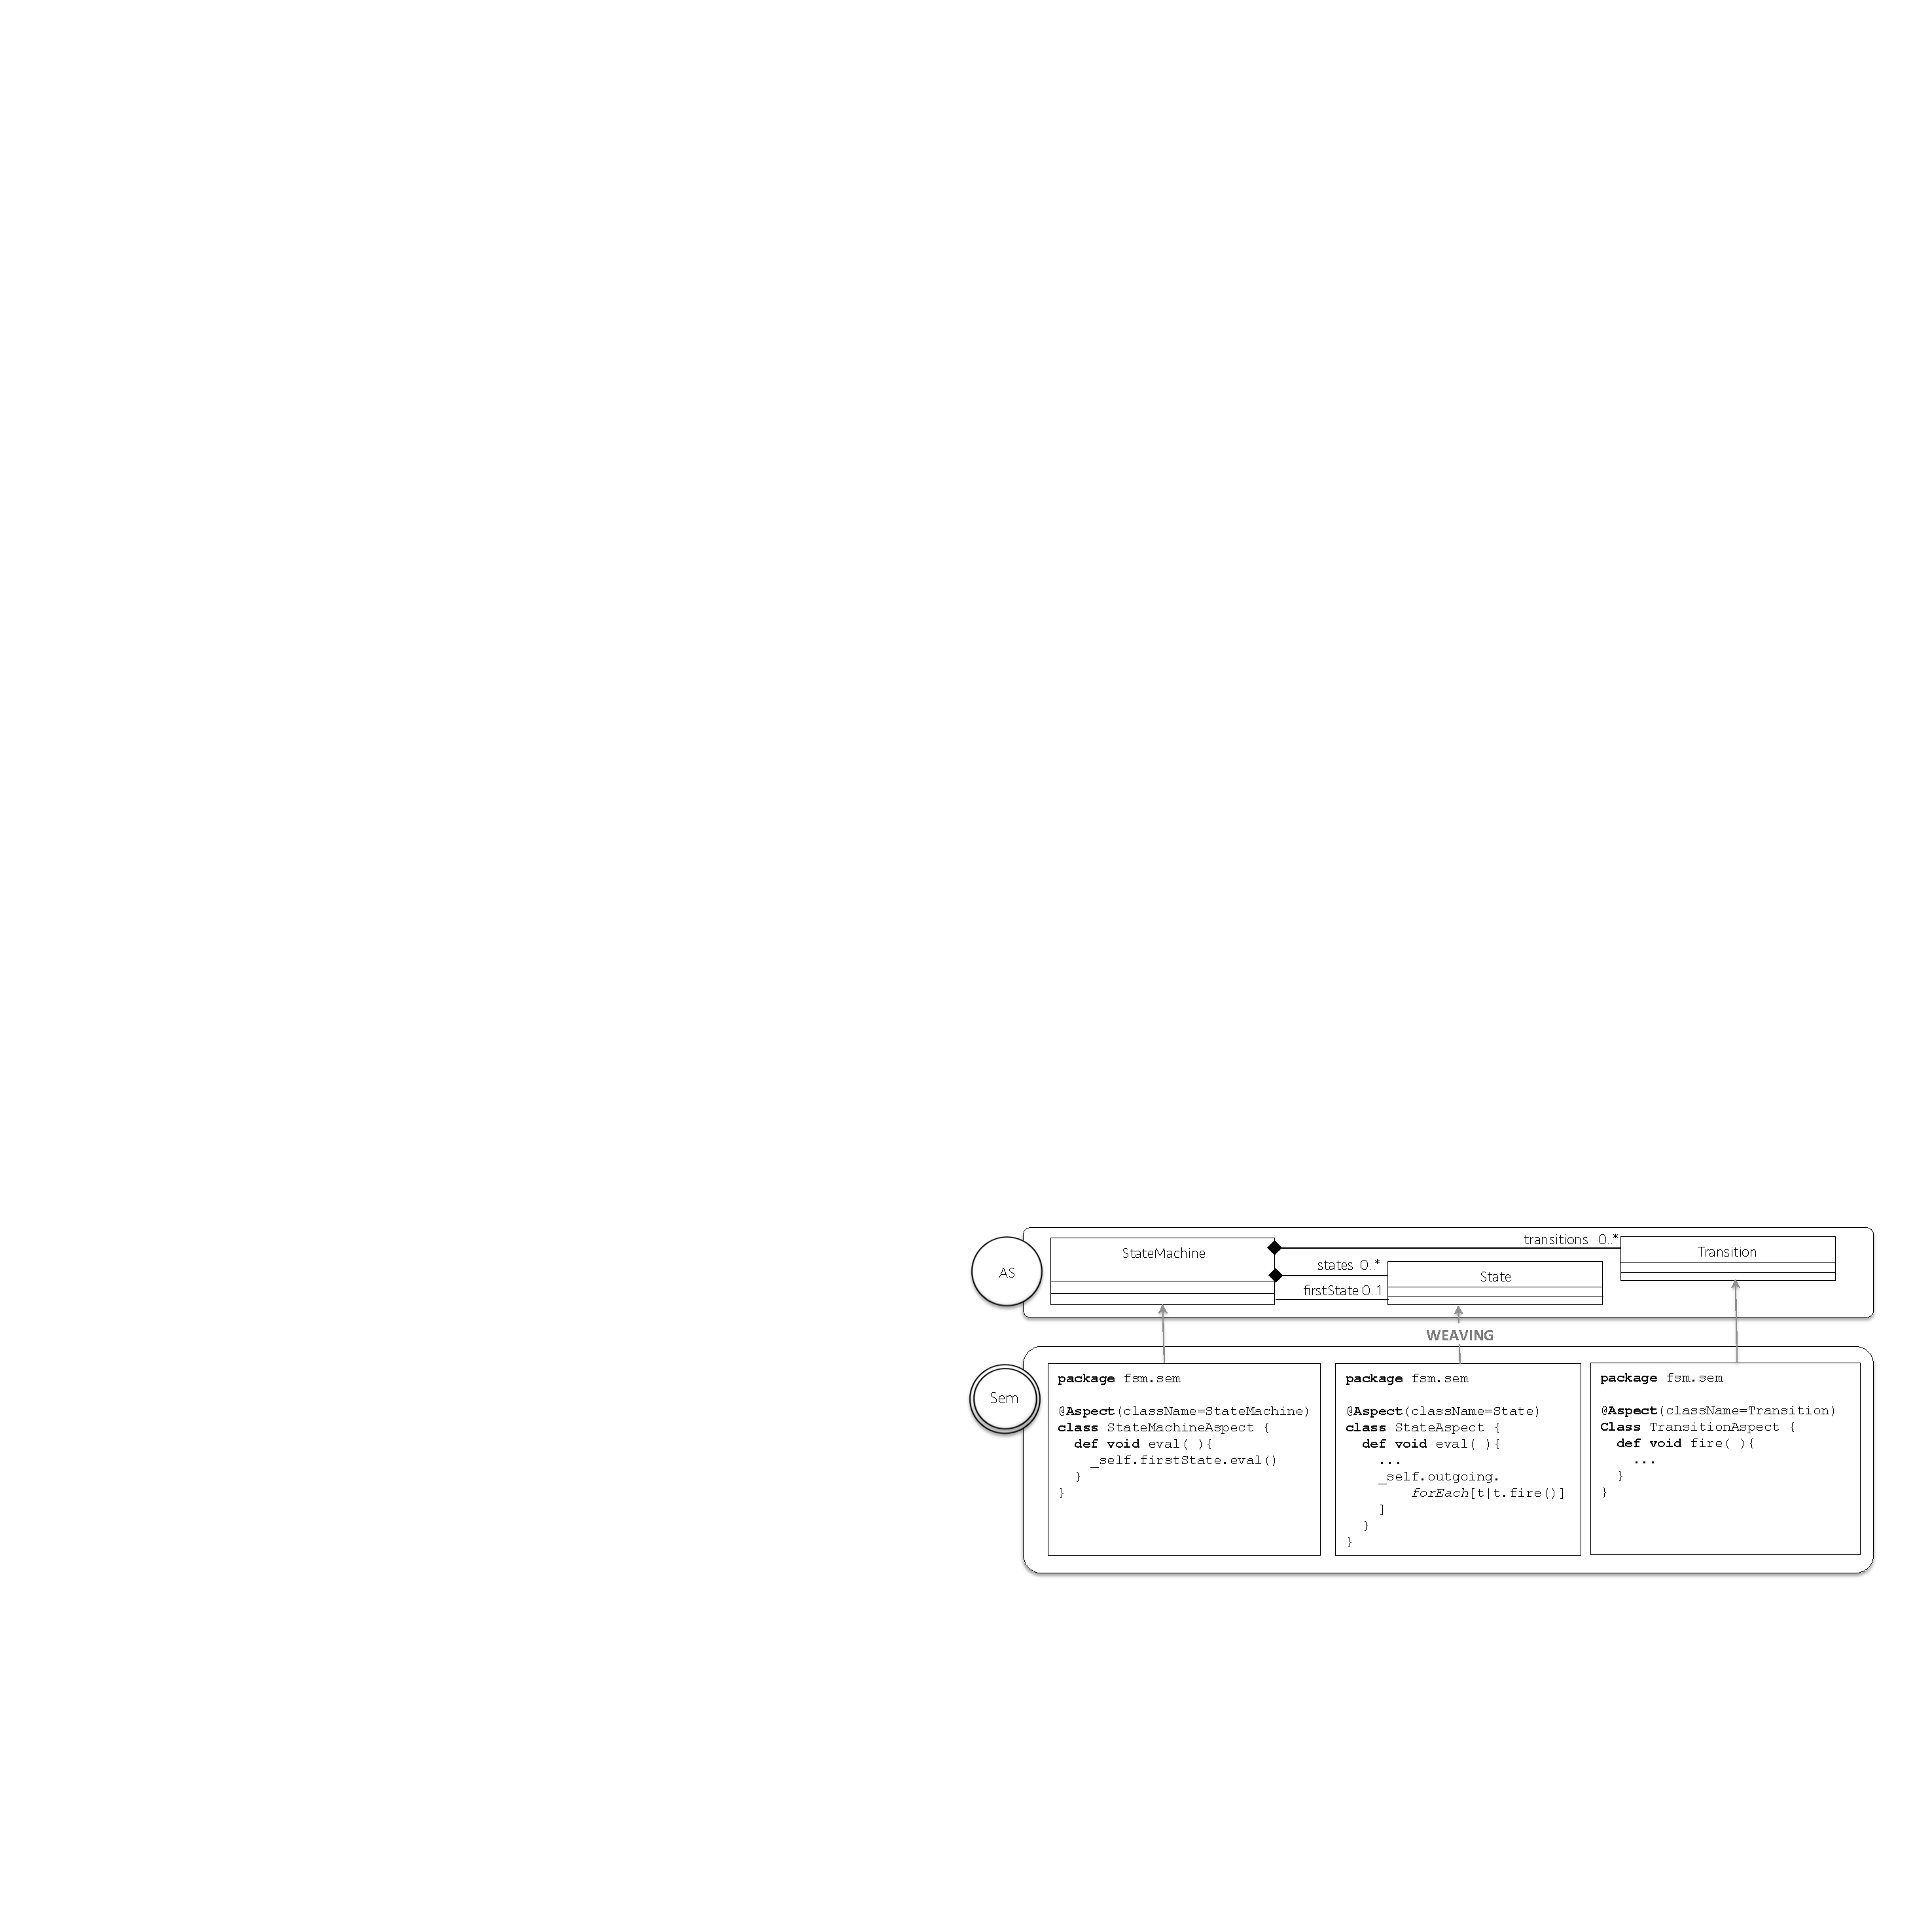
\includegraphics[width=1\linewidth]{images/k3-example-fig}
\caption{A simple DSL for finite state machines}
\label{fig:k3-example}
\end{figure}

%As said above, we use Melange to integrate and execute the definitions of the abstract syntax and semantics of a DSL. Melange is a language for modeling in the large that facilitates the integration of the different artifacts that compose the specification of a DSL. Listing \ref{lst:fsm} illustrates the use of Melange. At the left we have an abstract representation of a language that is composed of a metamodel and three aspects implementing the semantics. At the right of the figure we have the corresponding Melange script.
 
%\vspace{4mm}
%\begin{lstlisting}[caption=Melange script for a simple FSM language, label=lst:fsm]
%language FSM {
%    syntax "fsm.mm/models/fsm.ecore"
%    
%    with fsm.sem.StateMachineAspect
%    with fsm.sem.StateAspect
%    with fsm.sem.TransitionAspect
%}
%\end{lstlisting}

%\begin{figure}
%\centering
%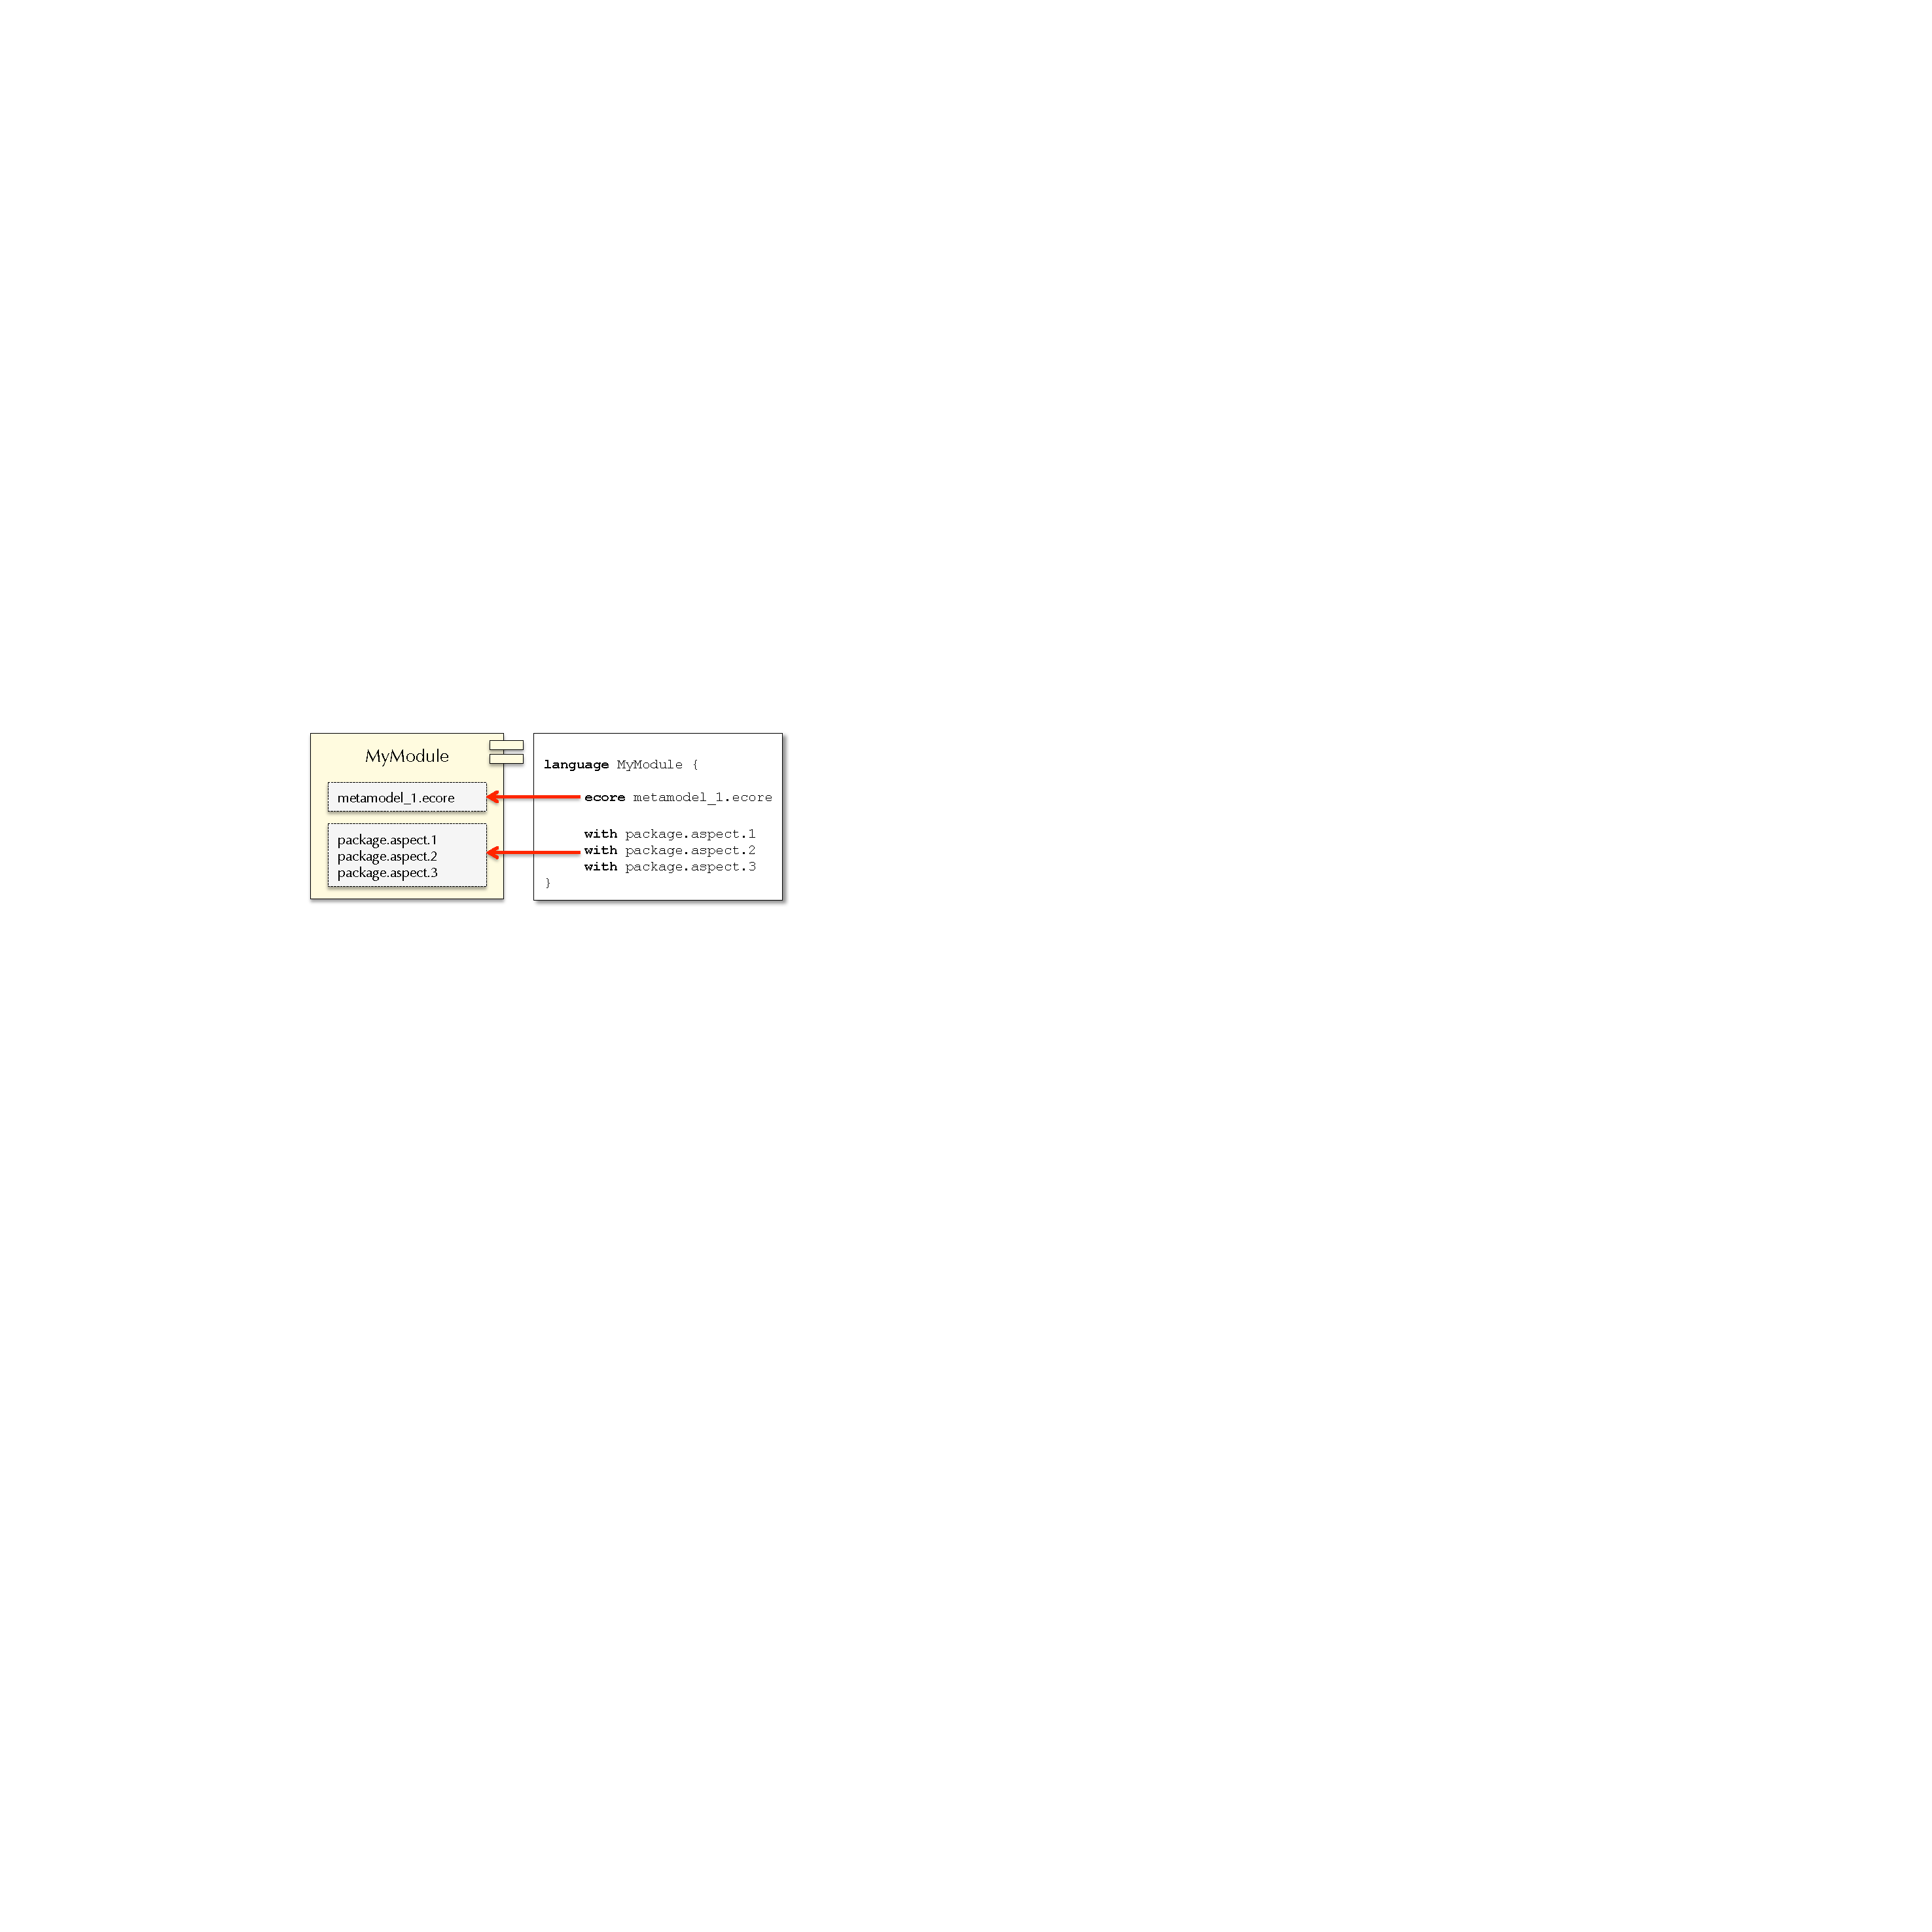
\includegraphics[width=0.8\linewidth]{images/module-melange}
%\caption{Using Melange for weaving metamodels and aspects}
%\label{fig:module-melange}
%\end{figure}
